\newcommand{\TP}{\ensuremath{\mathcal{M}}\xspace}			% Timed Payment
\newcommand{\TL}{\ensuremath{L}\xspace}														% Time Lottery
\newcommand{\DTL}{\ensuremath{\mathcal{L}}\xspace}									% Degenerated Time Lottery

\newcommand{\TLI}{\ensuremath{\mathcal{A}}\xspace}							% compound time lottery A
\newcommand{\TLII}{\ensuremath{\mathcal{B}}\xspace}							% compound time lottery B

\newcommand{\TLa}{\ensuremath{\TL_a}\xspace}							% time lottery a
\newcommand{\TLb}{\ensuremath{\TL_b}\xspace}							% time lottery b
\newcommand{\TLc}{\ensuremath{\TL_c}\xspace}							% time lottery c

\newcommand{\gra}{\ensuremath{\gr_a}\xspace}			% growth rate of time lottery a
\newcommand{\grb}{\ensuremath{\gr_b}\xspace}			% growth rate of time lottery b
\newcommand{\grc}{\ensuremath{\gr_c}\xspace}			% growth rate of time lottery c

\newcommand{\Dto}{\ensuremath{\Delta t_0}\xspace}
\newcommand{\tI}{\ensuremath{t_1}\xspace}
\newcommand{\Dtt}{\ensuremath{\Delta t_2}\xspace}
\newcommand{\tII}{\ensuremath{t_2}\xspace}

\newcommand{\gI}{\ensuremath{g_{\TP_1}}\xspace}
\newcommand{\gII}{\ensuremath{g_{\TP_2}}\xspace}
\newcommand{\ga}{\ensuremath{g_a}\xspace}
\newcommand{\gb}{\ensuremath{g_b}\xspace}
\newcommand{\DTLgr}{\ensuremath{g_{\DTL}}\xspace}


\begin{frame}{Commercial Break : Risk Preferences in Time Lotteries}{Full paper at: \url{bit.ly/TimeLotteries}}
% \ft{What is a Time Lottery?}
% \setbeamertemplate{itemize items}[triangle]
\setbeamercovered{invisible}
% Full paper at: \url{bit.ly/TimeLotteries}

\begin{columns}[T]
\column{0.4\textwidth}
\bi
\item Known payment amount: \Dx
\item Two possible payment times\\
% \bi
earlier	\tI \\
later \tII ($>$ \tI)
% \ei
\item Probability $0 \leq p \leq 1$ to receive \Dx earlier at \tI \\
($1-p$ later at \tII)
% \uncover<2->{
\item Every time lottery \TL defines a unique timed payment \DTL: \Dx is received with certainty at the expected payment time $\EA{t} = p\tI + \left(1-p\right)\tII$
% }
\ei
\column{0.6\textwidth}
\vspace{1cm}
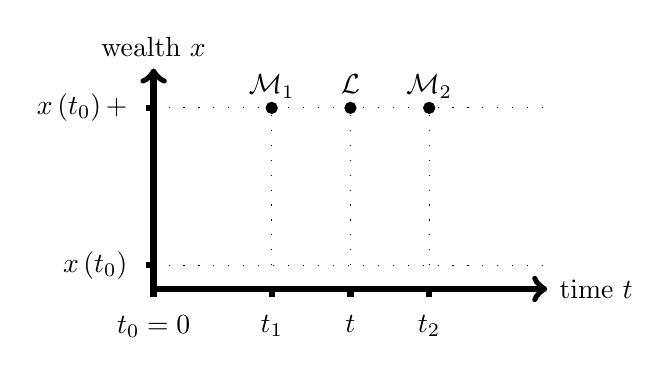
\begin{tikzpicture}[scale=.5]
	% every node/.style={draw,shape=circle,fill=blue},
	>=stealth																						% style of arrow tips
	]
		\draw [dash pattern=on \pgflinewidth off 5pt] (0,0) -- (10,0);
		\draw [dash pattern=on \pgflinewidth off 5pt] (0,4) -- (10,4);
		\draw [->, line width=0.8mm] (0,-0.6) -- (10,-0.6)	node[right,xshift=0pt]	{time $t$};
		\draw [->, line width=0.8mm] (0,-0.6) -- (0,5) 		node[above,yshift=0pt]	{wealth $x$};

		\draw[-,line width=0.8mm] (0,-0.8)--(0,-0.6) node[below, yshift=-5pt]{$t_0 = 0$};
		\draw[-,line width=0.8mm] (3,-0.8)--(3,-0.6) node[below, yshift=-5pt]{$\tI$};
		\draw[-,line width=0.8mm] (7,-0.8)--(7,-0.6) node[below, yshift=-5pt]{$\tII$};

		\draw[-,line width=0.8mm] (-0.2,0)--(0,0) node[left, xshift=-5pt]{$x\left(t_0\right)$};
		\draw[-,line width=0.8mm] (-0.2,4)--(0,4) node[left, xshift=-5pt]{$x\left(t_0\right) + \Dx$};

		\draw [dash pattern=on \pgflinewidth off 5pt] (3,0) -- (3,4) node [above] at (3,4)	{$\TP_1$};
		\filldraw[black] (3,4) circle (4pt);
% 	\uncover<2->{
		\draw[-,line width=0.8mm] (5,-0.8)--(5,-0.6) node[below, yshift=-5pt]{$\EA{t}$};
		\draw [dash pattern=on \pgflinewidth off 5pt] (5,0) -- (5,4) node [above] at (5,4)	{\DTL $\vphantom{\TP_1}$};
		\filldraw[black] (5,4) circle (4pt);
% 	}
		\draw [dash pattern=on \pgflinewidth off 5pt] (7,0) -- (7,4) node [above] at (7,4)	{$\TP_2$};
		\filldraw[black] (7,4) circle (4pt);

		\coordinate (origin) at (0,0);
		\coordinate (x_t1) at (3,4);
		\coordinate (exp_t) at (5,4);
		\coordinate (x_t2) at (7,4);
		\coordinate (bogus) at (4.2,4);

% 		\draw [loosely dotted,line width=0.4mm] (origin) -- (x_t1) node[anchor=east,pos=0.85] {};
%		\draw [line width=0.4mm]	(origin) -- (bogus)	node[anchor=east,pos=0.85] {\EAgr};
% 		\draw [loosely dashed,line width=0.4mm] (origin) -- (exp_t) node[anchor=west,pos=.85,xshift=5pt] {};
% 		\draw [loosely dotted, line width=0.4mm] (origin) -- (x_t2) node[anchor=west,pos=0.85,xshift=5pt] {};
\end{tikzpicture}
\end{columns}
\vspace{1em}
\bc
$\hookrightarrow$ Growth-optimal preferences vs EDUT preferences
\ec
%(Any degenerate time lottery \DTL is a timed payment)

\end{frame}